\documentclass[10pt, a4paper]{article}% size of txt = 10pt
\usepackage[top= 2cm,
			bottom = 2cm,
			left = 1.7cm,
			right = 1.7cm,
			footskip = 0.5cm,
			headsep = 0cm,
			headheight = 0cm
					]{geometry}
\usepackage{amsmath} % math packages
\usepackage{amsfonts}% math packages
\usepackage{amssymb} % math packages
\usepackage{graphicx} %package for including graphics
\usepackage{array}
\usepackage[thinlines]{easytable}
\usepackage{float}
\usepackage[section]{placeins}
\usepackage[hidelinks]{hyperref}
\usepackage[shortlabels]{enumitem}
\usepackage{svg}
\usepackage{bigstrut}
\usepackage{wrapfig,lipsum,booktabs}
\usepackage{subcaption}
\usepackage{xfrac}
\usepackage{pdfpages}
\usepackage{listings}
\usepackage{xcolor}


\usepackage{listings}
\usepackage{color} %red, green, blue, yellow, cyan, magenta, black, white
\definecolor{mygreen}{RGB}{28,172,0} % color values Red, Green, Blue
\definecolor{mylilas}{RGB}{170,55,241}

\definecolor{codegreen}{rgb}{0,0.6,0}
\definecolor{codegray}{rgb}{0.5,0.5,0.5}
\definecolor{codepurple}{rgb}{0.58,0,0.82}
\definecolor{backcolour}{rgb}{1,1,1}

\lstdefinestyle{mystyle}{
    backgroundcolor=\color{backcolour},   
    commentstyle=\color{codegreen},
    keywordstyle=\color{magenta},
    numberstyle=\tiny\color{codegray},
    stringstyle=\color{codepurple},
    basicstyle=\ttfamily\footnotesize,
    breakatwhitespace=false,         
    breaklines=true,                 
    captionpos=b,                    
    keepspaces=true,                 
    numbers=left,                    
    numbersep=5pt,                  
    showspaces=false,                
    showstringspaces=false,
    showtabs=false,                  
    tabsize=2
}
\lstset{style=mystyle}


%date format
\def\mydate{\leavevmode\hbox{\twodigits\day.\twodigits\month.\the\year}}
\def\twodigits#1{\ifnum#1<10 0\fi\the#1}

\usepackage{indentfirst}
\setlength{\parindent}{1cm}

\makeatletter
\newcommand{\thickhline}{%
    \noalign {\ifnum 0=`}\fi \hrule height 2pt
    \futurelet \reserved@a \@xhline
}
\newcolumntype{"}{@{\hskip\tabcolsep\vrule width 2pt\hskip\tabcolsep}}
\makeatother
\newcolumntype{?}{!{\vrule width 2pt}}
%%DOC ENVIROMENT%%%%%%%%%%%%%%%%%%%%%%%
\begin{document}
%Title 
\begin{flushleft}%% left justification
	\textbf{\Large{MKC-PKS: Úkol č. 2}}\hfill Filip Paul\\
	\large{Transportní a síťová vrstva UDP/TCP/IP \hfill\mydate}
\end{flushleft}
\section*{\large{\textbf{Přenosový tok protokolu plovoucího okna:}}}
	\begin{itemize}[label={}]
		\item \textbf{Zadání:}\\
		Předpokládejte spoj za použití linek 1Gb/s s celkovou délkou optického vlákna 100km. Komunikace
		probíhá pomocí paketů  velikosti 1500B. Vypočtěte dosažitelný přenosový tok při použití protokolu
		plovoucího okna, jehož velikost je 10 paketů.
		Celkové zpoždění při zpracování paketů a čekání ve frontách ve všech vnitřních uzlech sítě je 200\,$\mu$s v
		jednom směru (nezahrnuje dobu šíření signálu v optickém vláknu).\\

		\item \textbf{Vypracování:}\\
		\begin{figure}[ht!]
			\centering
			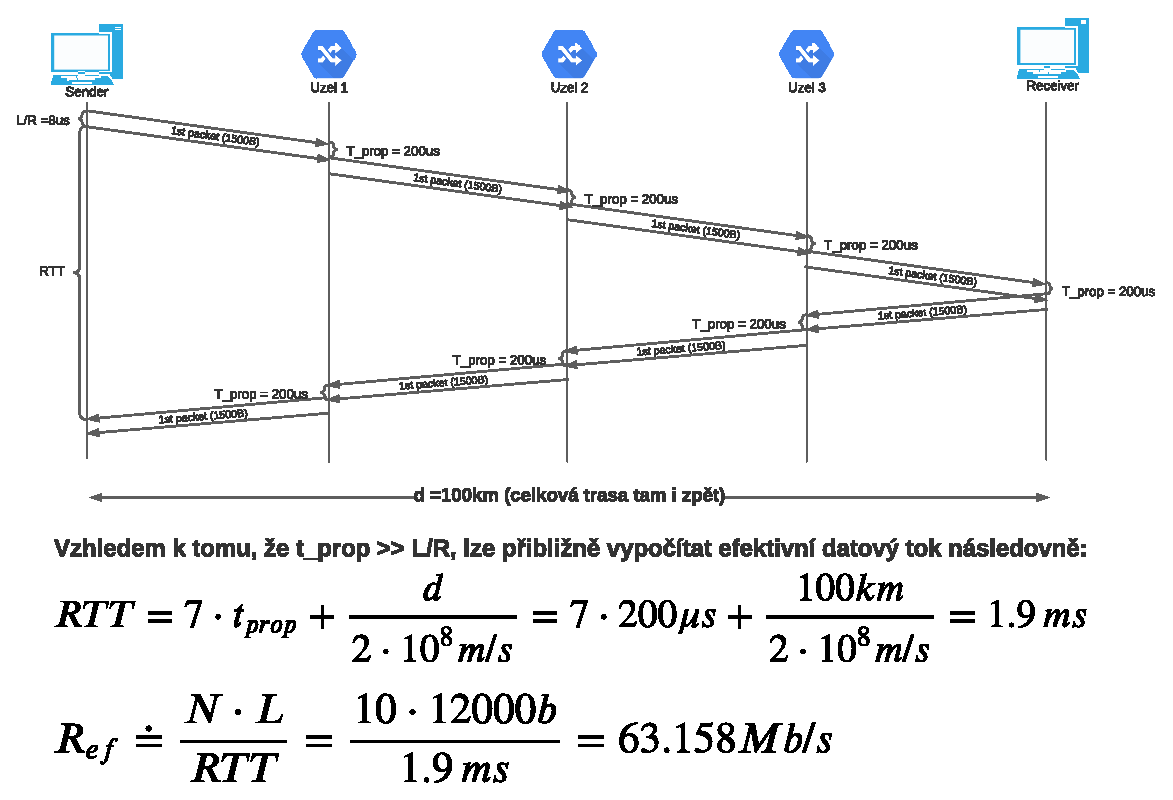
\includegraphics[width = 0.85\textwidth]{plov_okno.eps}
		\end{figure}
				
	\end{itemize}

\section*{\large{\textbf{Přenosový tok protokolu plovoucího okna:}}}
	\begin{itemize}[label={}]

		\item \textbf{Zadání:}
			V tabulce je zachycena komunikace uzlu protokolem TCP. Napište, k čemu došlo a jaká bude reakce
			odesílající stanice?
		
		\item \textbf{Vypracování:}\\\\
		\begin{minipage}{0.4\textwidth}
			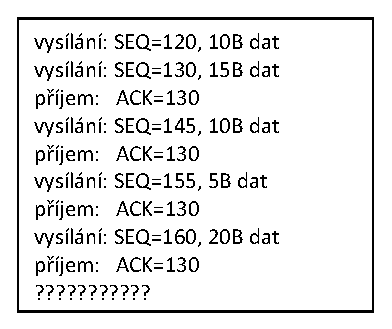
\includegraphics{TCP_table.eps}
		\end{minipage}
		\begin{minipage}{0.58\textwidth}
			\vspace{-2.2cm}
			Odesílání 1. packetu (SEQ 120; 10B) proběhlo v pořádku. Další packety však už
			nebyly potvrzeny. Nyní záleží na tom, zda komunikace proběhla ještě před vypršením timeoutu.
			Pokud komunikace proběhla v jednou timeout okně, tak lze zaslat "fast retransmitt" zprávy (SEQ = 130;15B).
			V případě úspěšného retransmittu přijde ACK = 180. Pokud však vyprší timeout je nutné
			zaslat znova vše kromě 1. zprávy.

		\end{minipage}
	\end{itemize}
	\clearpage

	\section*{\large{\textbf{Směrovací tabulky:}}}
	\begin{itemize}[label={}]

		\item \textbf{Zadání:}
		Vhodně zvolte adresy všech rozhraní směrovačů (adresy v Internetu si zvolte). Napište směrovací
		tabulku pro směrovače RT1 a RT2. Uvažujte agregaci adres a tzv. výchozí cestu (default route).
		
		\item \textbf{Vypracování:}\\\\
		\begin{figure}[ht!]
			\centering
			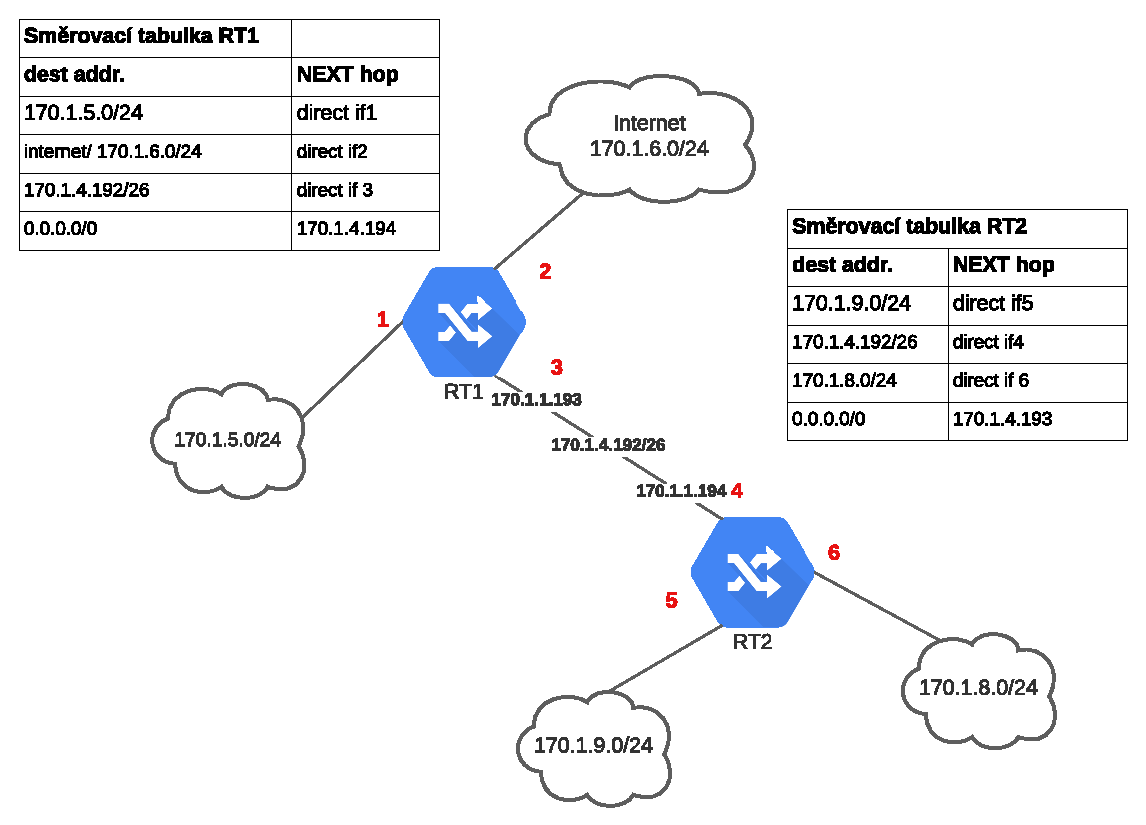
\includegraphics[width = 1\textwidth]{tabulky.eps}
		\end{figure}
	\end{itemize}
	

\end{document}